\subsection{Class counts, transitions, and outcome associations}

The call distinguishes class-conditioned router features from the proportion
of reasoning assigned to each class (24:41--29:57). The following plots use
\emph{sampled sentence shares}: the number of labelled sentences of a class
divided by the number of labelled sentences in that attempt. An observed
zero share is retained; unlabelled sentences are never assigned a class.
These are estimates from the sampling protocol, not complete-sequence class
fractions. Each source problem contributes only its sample-zero attempt;
benchmark comparisons retain their separate denominators. Attempts with no
labelled sentences are excluded.

\begingroup\scriptsize\setlength{\tabcolsep}{4pt}
\begin{longtable}{@{}lrrrrrrrr@{}}
\caption{Mean sampled sentence share (percent), with equal weight per labelled attempt. Empty-label attempts are excluded; absent classes in an observed sample have zero share. These are not full-corpus class proportions.}\label{tab:class-shares}\\
\toprule
Dataset & Attempts & Read & Analyze & Plan & Implement & Explore & Verify & Monitor \\
\midrule\endfirsthead
\multicolumn{9}{l}{\textit{Continued from previous page}}\\
\toprule
Dataset & Attempts & Read & Analyze & Plan & Implement & Explore & Verify & Monitor \\
\midrule\endhead
\bottomrule\endfoot
MATH-500 & 499 & 8.9 & 19.5 & 9.3 & 29.3 & 4.1 & 11.8 & 17.1 \\
AIME24 & 30 & 6.7 & 33.9 & 2.9 & 28.3 & 7.0 & 14.4 & 6.8 \\
AIME25 & 30 & 5.7 & 33.2 & 4.8 & 27.9 & 6.7 & 13.4 & 8.3 \\
Olympiad & 675 & 6.9 & 26.8 & 6.0 & 29.7 & 6.4 & 13.2 & 11.0 \\
AMC23 & 40 & 6.6 & 25.9 & 5.8 & 32.0 & 3.8 & 15.2 & 10.6 \\
Minerva & 272 & 9.4 & 19.8 & 8.4 & 21.8 & 7.7 & 10.3 & 22.6 \\
\end{longtable}\endgroup


\begin{figure}[p]
\centering
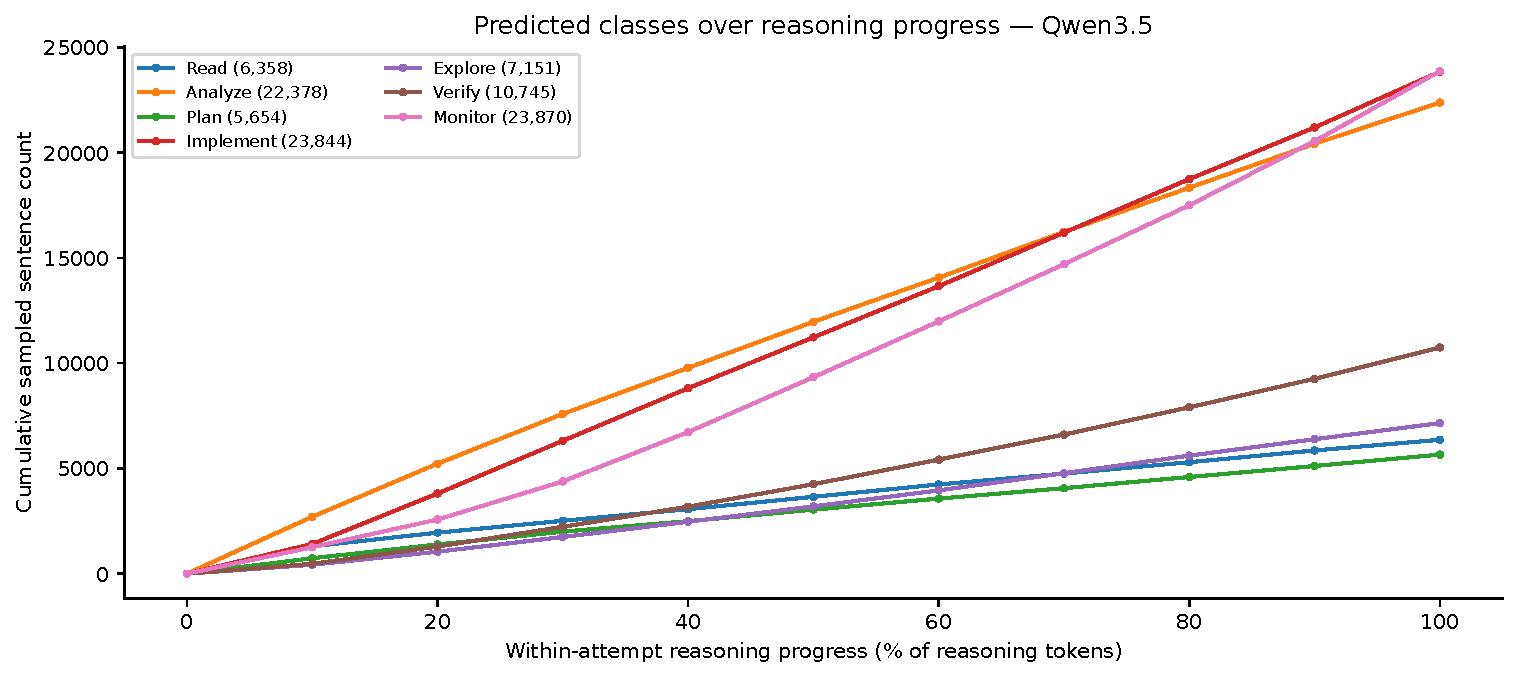
\includegraphics[width=\linewidth]{figures/qwen_class_cumulative.pdf}
\caption{Cumulative counts of sampled sentences by predicted class, pooled
across benchmarks. Counts start at zero; a sentence is counted when its last
reasoning token is reached. Progress is normalized by each attempt's full
reasoning-token length, unlike the absolute windows in
Figure~\ref{fig:qwen-position}. Legend totals equal the rightmost endpoints.
These are raw sampled counts, not cumulative percentages or estimates of
full-corpus counts; longer traces and benchmark sampling quotas affect them.}
\label{fig:class-cumulative}
\Description{Predicted sentence classes are summarized from sampled labels; the caption defines the counts, denominators, and outcomes.}
\end{figure}

\begin{figure}[p]
\centering
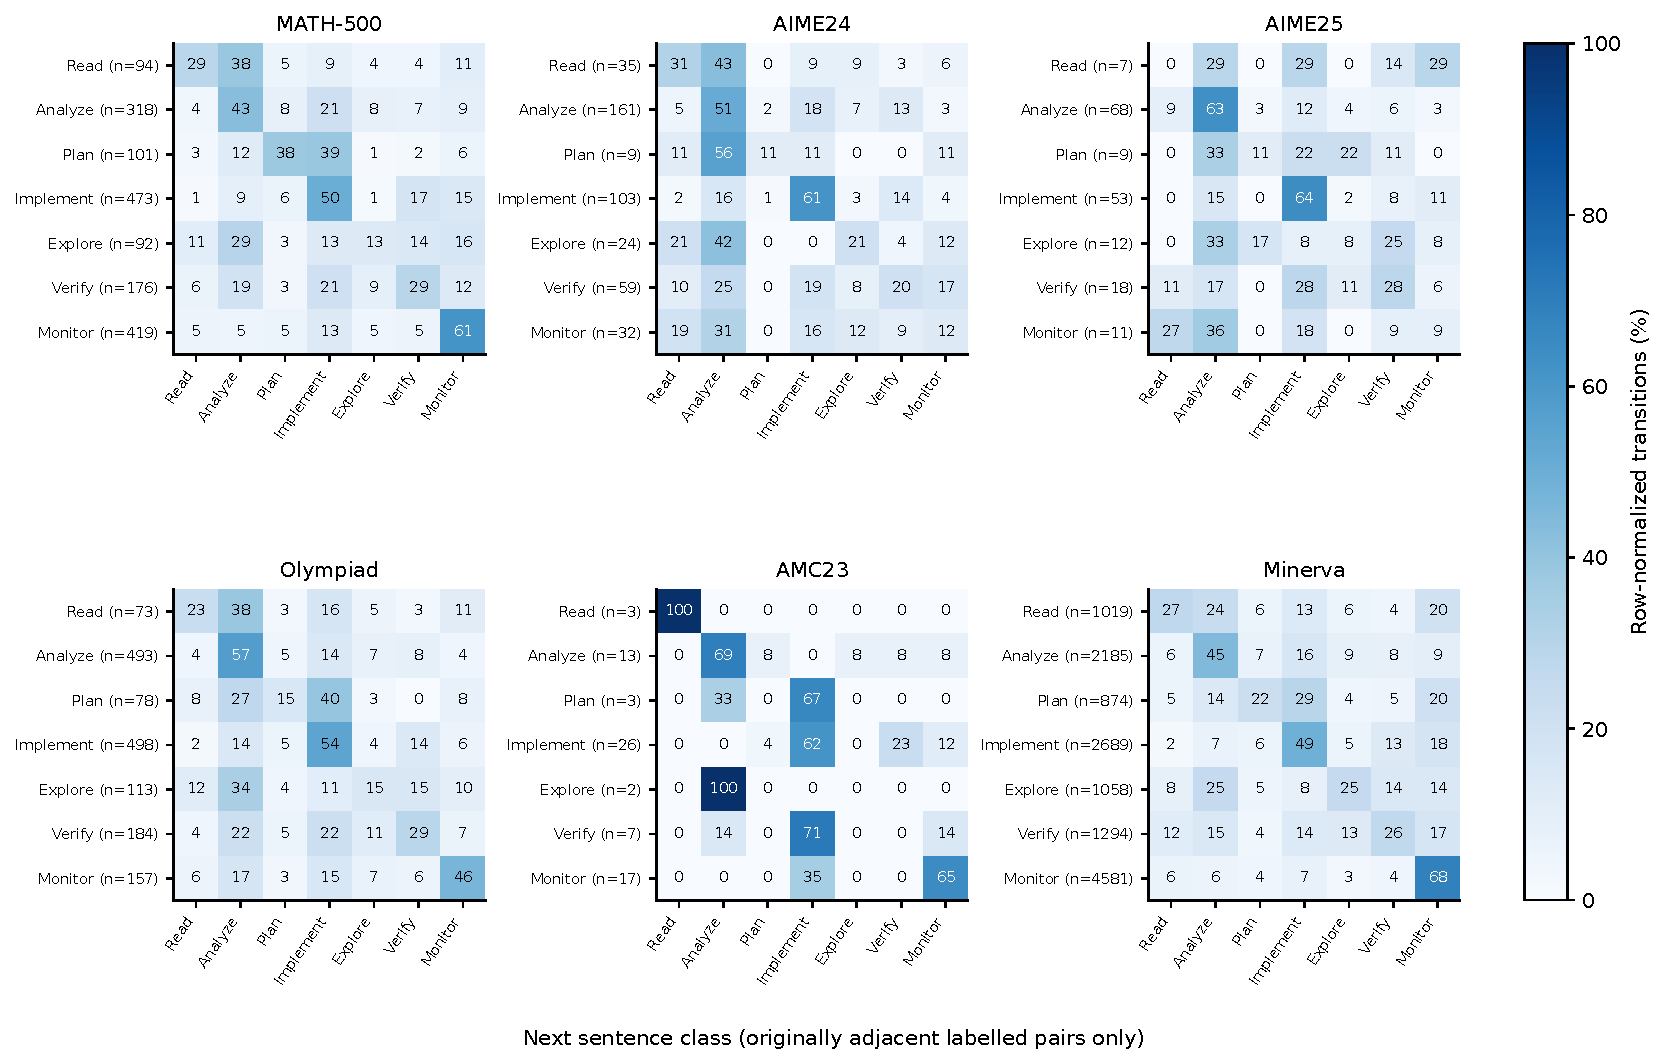
\includegraphics[width=\linewidth]{figures/qwen_class_transitions.pdf}
\caption{Observed class-state transitions by benchmark. Rows are the current
class, columns the next class; cells are row percentages and row labels give
pair counts. Only originally consecutive sentence indices with both labels
are counted. Gaps in sampling are never bridged. Self-transitions are retained;
empty rows are undefined. This describes the observed adjacent-pair sample,
not the complete transition process or an effect of changing state.}
\label{fig:class-transitions}
\Description{Predicted sentence classes are summarized from sampled labels; the caption defines the counts, denominators, and outcomes.}
\end{figure}

\begin{figure}[p]
\centering
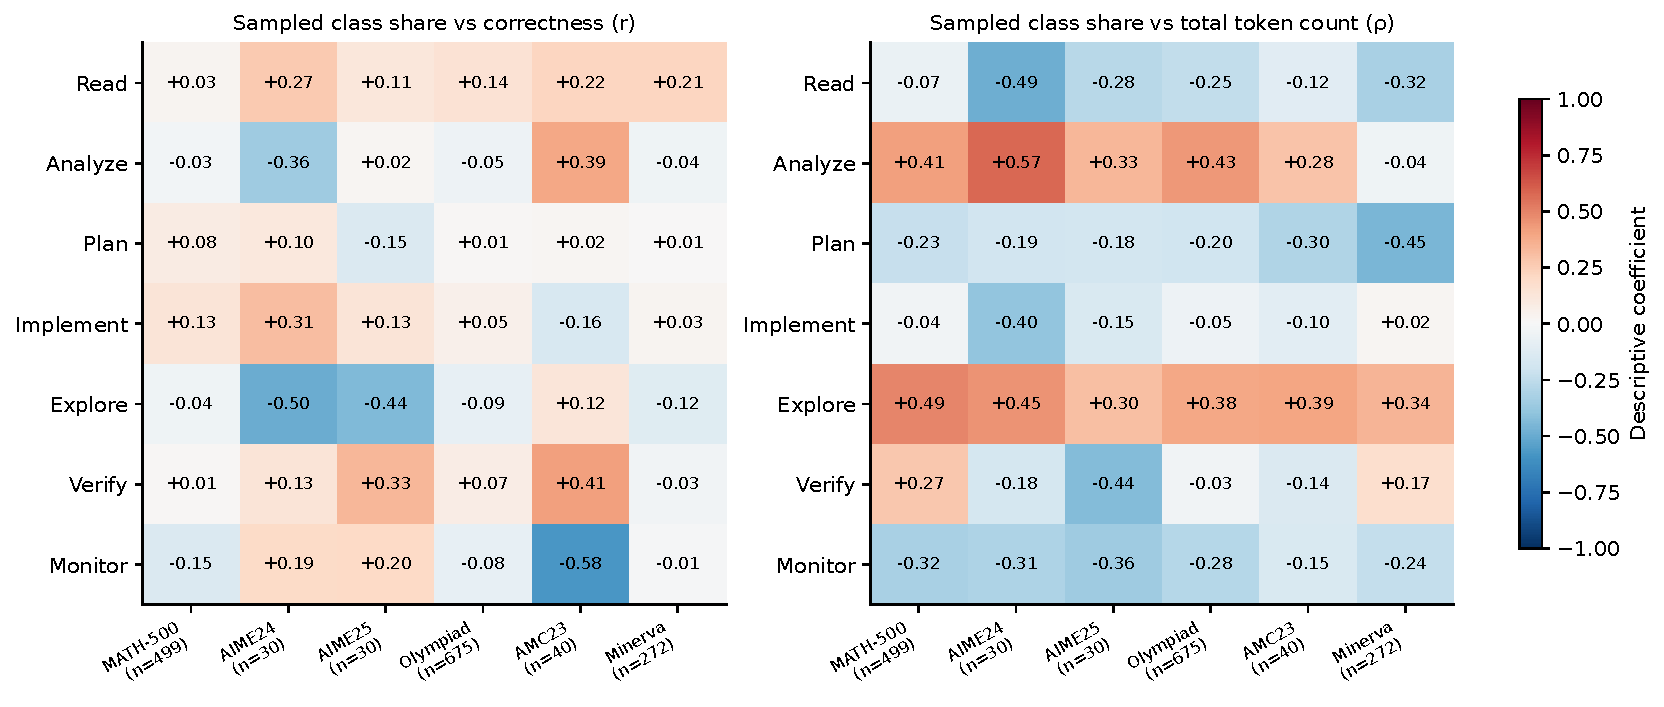
\includegraphics[width=\linewidth]{figures/qwen_class_share_correlations.pdf}
\caption{Sampled class proportions versus whole-attempt correctness
(point-biserial $r$) and total continuation-token count (Spearman $\rho$).
All labelled attempts enter each class, including observed zero proportions.
These differ from correlations of router features within class-selected
tokens. No significance claim is made; class shares sum to one and cannot
be interpreted as independent effects.}
\label{fig:class-share-correlations}
\Description{Predicted sentence classes are summarized from sampled labels; the caption defines the counts, denominators, and outcomes.}
\end{figure}

\begin{figure}[p]
\centering
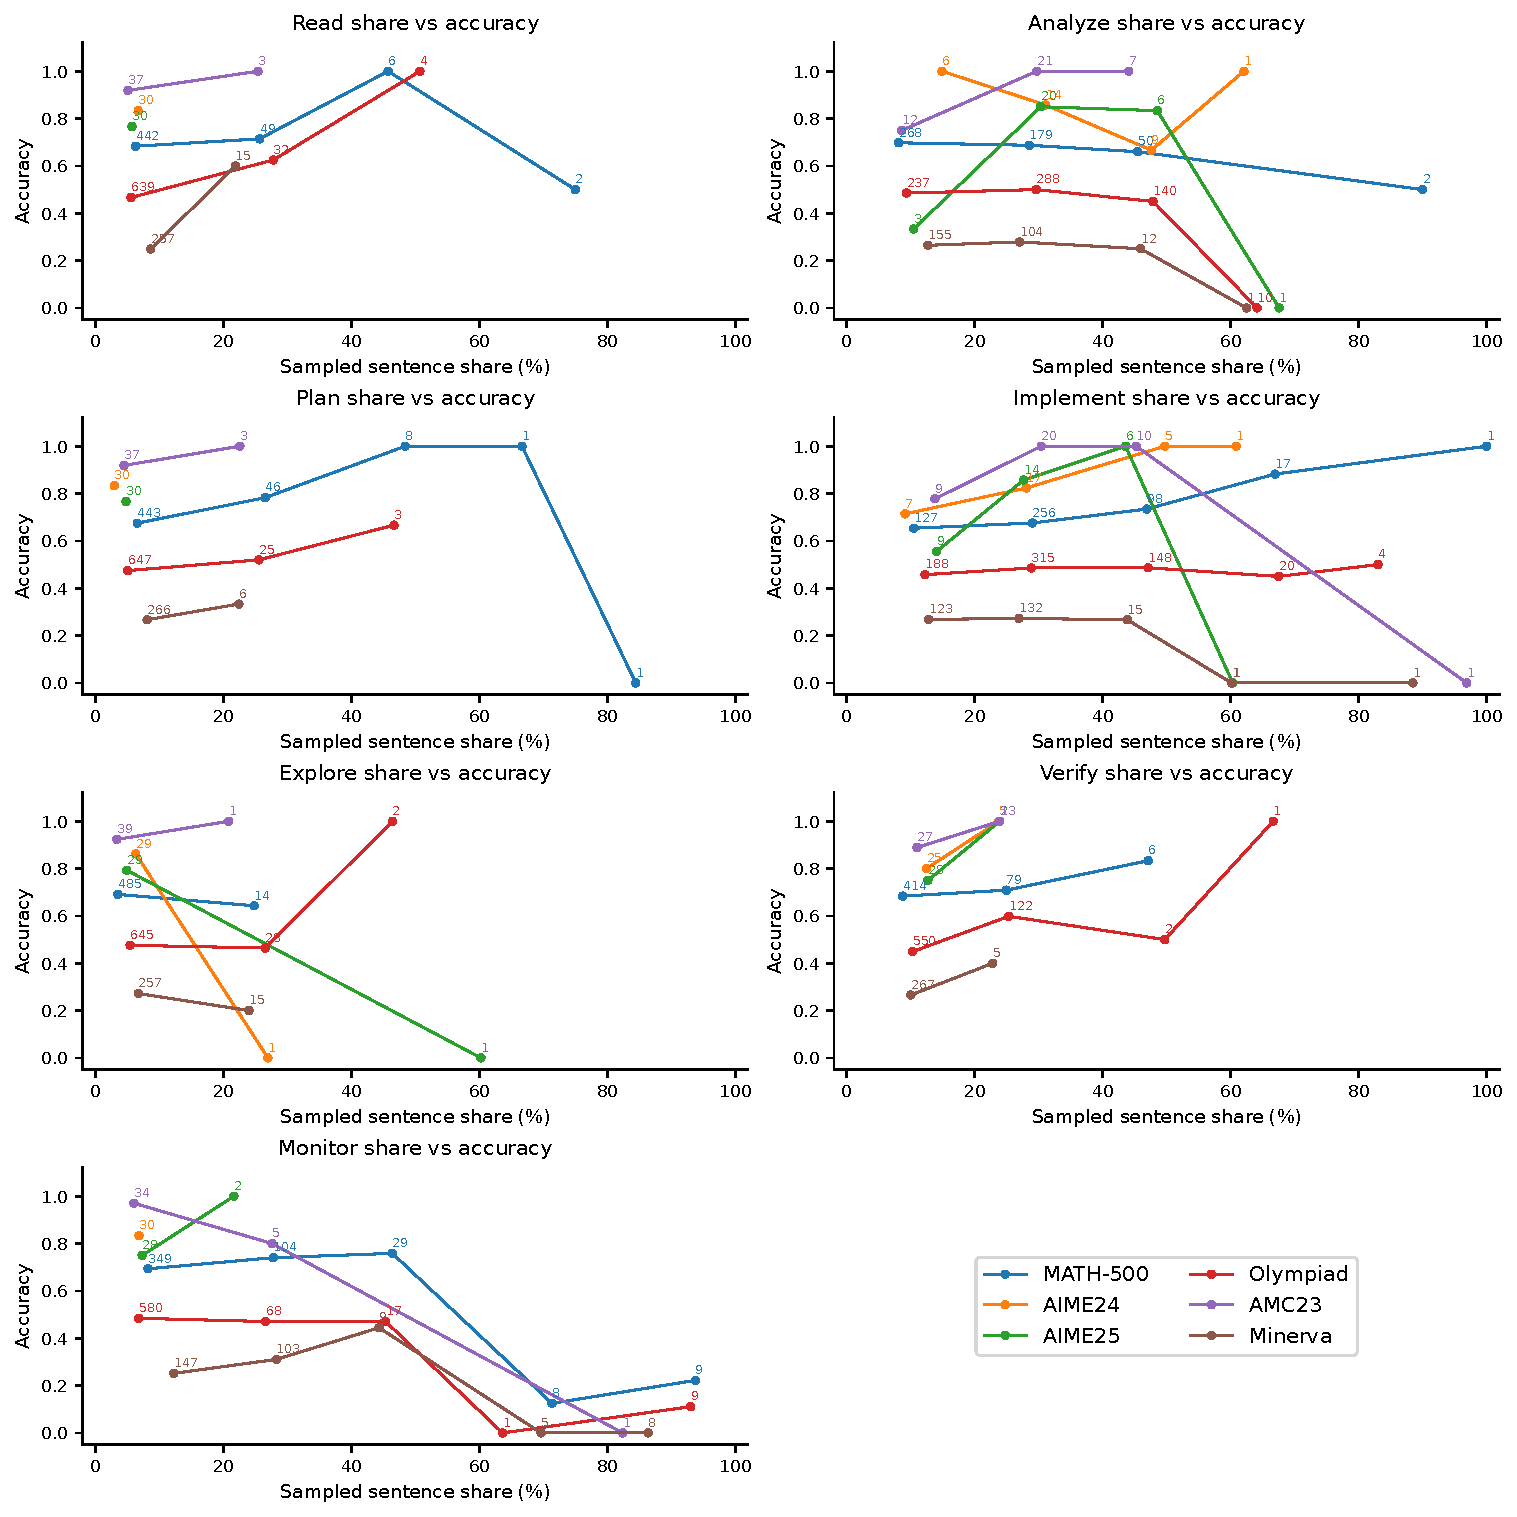
\includegraphics[width=\linewidth]{figures/qwen_class_share_accuracy.pdf}
\caption{Actual outcome levels versus sampled class proportions. Fixed share
bins are $[0,20)$, $[20,40)$, $[40,60)$, $[60,80)$, and $[80,100]$ percent.
Each point is at the mean observed share and shows accuracy; small labels give attempt counts. Empty
bins are omitted. Colours distinguish benchmarks; lines only connect
occupied bins. Sparse bins, sentence sampling, length, and difficulty can
explain apparent trends; these descriptive plots do not identify optimal
class proportions or a validated accuracy--length Pareto frontier.}
\label{fig:class-share-outcomes}
\Description{Predicted sentence classes are summarized from sampled labels; the caption defines the counts, denominators, and outcomes.}
\end{figure}

\begin{figure}[p]
\centering
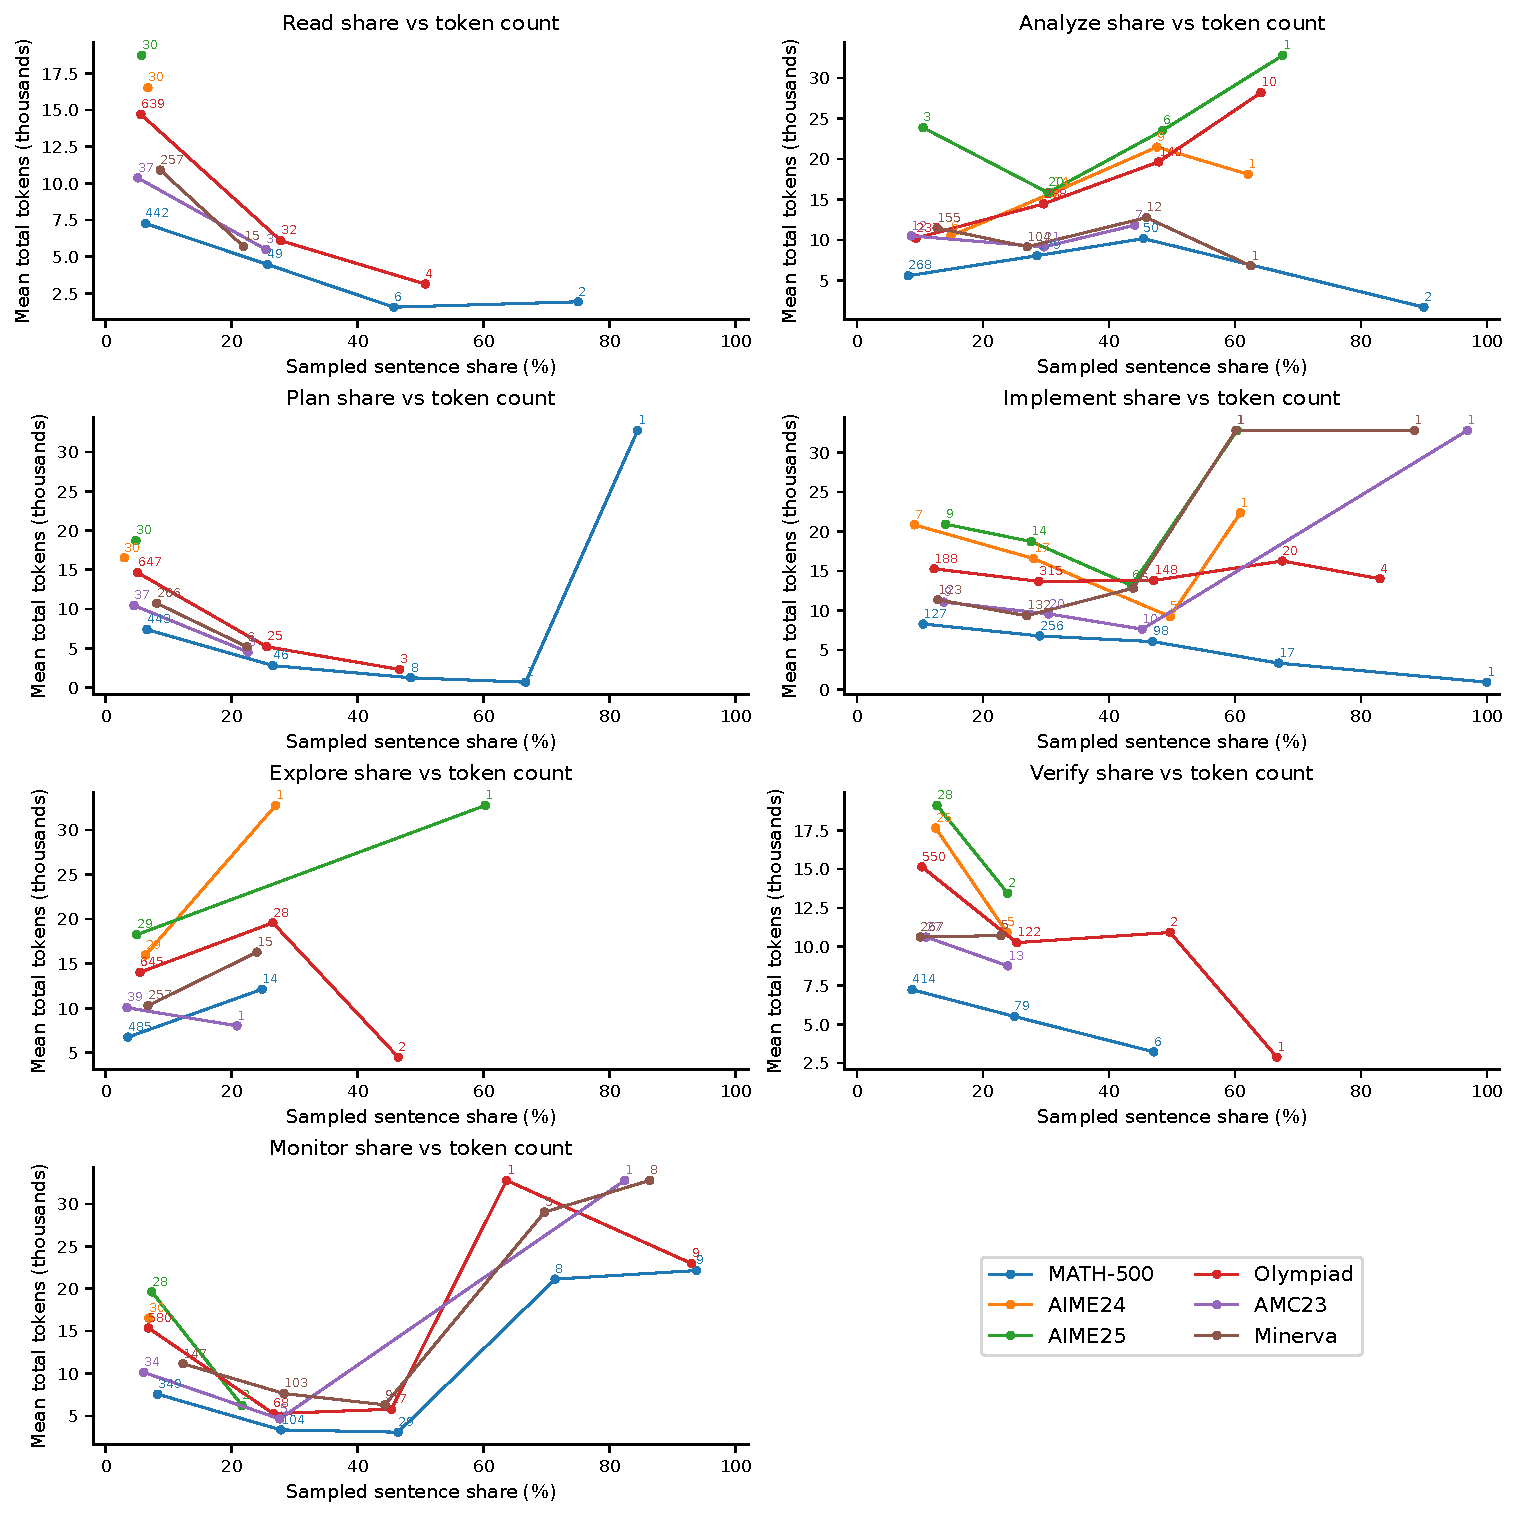
\includegraphics[width=.95\linewidth]{figures/qwen_class_share_tokens.pdf}
\caption{Mean total continuation tokens versus sampled class share. Bin
boundaries, colours, sample-count labels, and sampling limitations are as in
Figure~\ref{fig:class-share-outcomes}. Token count includes the final answer
and token-limit completions; lines are descriptive, not intervention effects.}
\label{fig:class-share-tokens}
\Description{Predicted sentence classes are summarized from sampled labels; the caption defines the counts, denominators, and outcomes.}
\end{figure}

Class-state dynamics remain descriptive. Relating complete transition paths
to correctness and interventions conditioned on those paths is future work,
as agreed at 29:32--30:20 and 45:23--48:10. The currently sampled labels do
not justify reconstructing missing transitions.
